% Impostazioni principali
\documentclass[t, compress, mathserif]{beamer}



%         ----------------------------------------------         %
%        /                                              \        %
%--------               START PREAMBLE                   --------%
%        \                                              /        %
%         ----------------------------------------------         %

% Titolo che appare nella prima slide del documento
\newcommand{\titolo}{Decision Tree of statistical tests}
\newcommand{\sottotitolo}{Choice of the method according to the purpose of the data} 

% Titolo che appare nella barra in basso di ogni slide, al centro
% Sono due variabili:
% * una puo' essere utilizzata per l'intero corso. Se impostata nel preambolo sovrascrive quella di seguito.
% * l'altra puo' identificare ciascun documento
\newcommand{\titolocompleto}{Statistics course - }
\newcommand{\titoloshort}{\titolo}

% Numero di capitolo o altro nome che appare in basso di ogni slide, vicino al numero di pagina
\newcommand{\numerocapitolo}{Appendix 1}

% Include il documento che contiene il preambolo

%%%%%%%%%%%%%%%%%%%%%%%%%%%%%%%%%%%%%%%%%%%%%%%%%%%%%%%%%%%%%%%%%%%%%%%%%%%%%%
%%%%%%%%%%%%%%%%%%%%%%%%%%%% VARIABILI DA DEFINIRE %%%%%%%%%%%%%%%%%%%%%%%%%%%
%%%%%%%%%%%%%%%%%%%%%%%%%%%%%%%%%%%%%%%%%%%%%%%%%%%%%%%%%%%%%%%%%%%%%%%%%%%%%%

% Titolo che appare nella barra in basso di ogni slide, al centro
% Se impostato ha la precedenza rispetto a quello di ogni singola slide

%\renewcommand{\titolocompleto}{}

% non c'e' newcommand{\sottotitolo} perche' viene definito in ogni slide
\newcommand{\data}{}



%%%%%%%%%%%%%%%%%%%%%%%%%%%%%%%%%%%%%%%%%%%%%%%%%%%%%%%%%%%%%%%%%%%%%%%%%%%%%%
%%%%%%%%%%%%%%%%%%%%%%%%%%%%%%%%%% PACKAGES %%%%%%%%%%%%%%%%%%%%%%%%%%%%%%%%%%
%%%%%%%%%%%%%%%%%%%%%%%%%%%%%%%%%%%%%%%%%%%%%%%%%%%%%%%%%%%%%%%%%%%%%%%%%%%%%%
\usepackage[latin1]{inputenc}   
\usepackage{graphicx}
\usepackage{rotating}
\usepackage{rotfloat}
\usepackage{color}
\usepackage{colortbl}
\usepackage{../includeTex/floatflt}
\usepackage{tikz}
\usepackage{hyperref}
\usepackage{pgfpages} 
\usepackage{ifthen}
\usepackage{wasysym}
\usepackage{multirow}



%%%%%%%%%%%%%%%%%%%%%%%%%%%%%%%%%%%%%%%%%%%%%%%%%%%%%%%%%%%%%%%%%%%%%%%%%%%%%%
%%%%%%%%%%%%%%%%%%%%%%%%%%%% IMPOSTAZIONI GENERALI %%%%%%%%%%%%%%%%%%%%%%%%%%%
%%%%%%%%%%%%%%%%%%%%%%%%%%%%%%%%%%%%%%%%%%%%%%%%%%%%%%%%%%%%%%%%%%%%%%%%%%%%%%

% Beamer theme
%\usetheme{CambridgeUS}      
\usetheme{Madrid}      

% Immagini da visualizzare
\newcommand{\materiale}{minitab}

% Path delle immagini
\graphicspath{{../images/}}

% Per caricare le formule matematiche con il giusto font 
% Questo sostituisce l'opzione mathserif di documentclass (obsoleta) 
\usefonttheme[onlymath]{serif}      

     

%%%%%%%%%%%%%%%%%%%%%%%%%%%%%%%%%%%%%%%%%%%%%%%%%%%%%%%%%%%%%%%%%%%%%%%%%%%%%%
%%%%%%%%%%%%%%%%%%%%%%%%%%%%%%%%%%% COLORI %%%%%%%%%%%%%%%%%%%%%%%%%%%%%%%%%%%
%%%%%%%%%%%%%%%%%%%%%%%%%%%%%%%%%%%%%%%%%%%%%%%%%%%%%%%%%%%%%%%%%%%%%%%%%%%%%%

\definecolor{grigio}{rgb}{0.46,0.48,0.48}
\definecolor{giallo}{rgb}{1,0.84,0}
\definecolor{coolred}{rgb}{0.83,0.06,0.27}
\definecolor{arancio}{rgb}{0.97,0.46,0.09}
\definecolor{verde}{rgb}{0.25,0.78,0.25}
\definecolor{qblu}{rgb}{0.24,0.27,0.74}
\definecolor{azzurro}{rgb}{0.37,0.91,0.90}

\definecolor{grigio}{rgb}{0.46,0.48,0.48}
\definecolor{blu}{rgb}{0.25,0.28,0.78}

\definecolor{sfondoScopo}{rgb}{0.75,0.785,0.83}
\definecolor{darkred}{named}{qblu}
\definecolor{blue}{named}{qblu}

\setbeamercolor{scopo}{bg=sfondoScopo}
\setbeamercolor{section in toc}{fg=black,bg=white}
\setbeamercolor{alerted text}{fg=darkred!80!gray}
\setbeamercolor{palette primary}{fg=darkred!60!black,bg=gray!30!white}
\setbeamercolor{palette secondary}{fg=darkred!70!black,bg=gray!15!white}
\setbeamercolor{palette tertiary}{bg=darkred!80!black,fg=gray!10!white}
\setbeamercolor{palette quaternary}{fg=darkred,bg=gray!5!white}

\setbeamercolor{sidebar}{fg=darkred,bg=gray!15!white}
\setbeamercolor{palette sidebar primary}{fg=darkred!10!black}
\setbeamercolor{palette sidebar secondary}{fg=white}
\setbeamercolor{palette sidebar tertiary}{fg=darkred!50!black}
\setbeamercolor{palette sidebar quaternary}{fg=gray!10!white}

\setbeamercolor{titlelike}{parent=pallette primary,fg=darkred}
\setbeamercolor{frametitle}{bg=gray!10!white}
\setbeamercolor{frametitle right}{bg=gray!60!white}

\setbeamercolor{separation line}{}
\setbeamercolor{fine separation line}{}

%% Definizione dei colori da assegnare ai box
\setbeamercolor{postit}{fg=white,bg=qblu}
\setbeamercolor{postut}{fg=qblu,bg=gray!60!white}

%% Definizione dei colori per i diagrammi
\definecolor{bloccoIniziale}{rgb}{0.94,0.93,0.48}
\definecolor{bloccoFinale}{rgb}{0.86,0.25,0.27}
\definecolor{blocco}{rgb}{0.56,0.58,0.77}
\definecolor{bloccoSospeso}{rgb}{0.94,0.81,0.36}



%%%%%%%%%%%%%%%%%%%%%%%%%%%%%%%%%%%%%%%%%%%%%%%%%%%%%%%%%%%%%%%%%%%%%%%%%%%%%%
%%%%%%%%%%%%%%%%%%%%%%%%% STRUTTURA DELLE DIAPOSITIVE %%%%%%%%%%%%%%%%%%%%%%%%
%%%%%%%%%%%%%%%%%%%%%%%%%%%%%%%%%%%%%%%%%%%%%%%%%%%%%%%%%%%%%%%%%%%%%%%%%%%%%%

% Intestazione
\setbeamertemplate{headline}
{
  \leavevmode%
  \hbox{%
  \begin{beamercolorbox}[wd=.5\paperwidth,ht=2.25ex,dp=1ex,right]{section in head/foot}%
    \usebeamerfont{section in head/foot}\insertsectionhead\hspace*{2ex}
  \end{beamercolorbox}%
  \begin{beamercolorbox}[wd=.5\paperwidth,ht=2.25ex,dp=1ex,left]{subsection in head/foot}%
    \usebeamerfont{subsection in head/foot}\hspace*{2ex}\insertsubsectionhead
  \end{beamercolorbox}}%
  \vskip0pt%
}

% Pie' di pagina
\setbeamertemplate{footline}
{
  \hbox{%
    \begin{beamercolorbox}[wd=.20\paperwidth, ht = 2.25ex, dp = 1ex, center]{palette sidebar secondary}%
      \usebeamerfont{author in head/foot}%\insertshortauthor~~(\insertshortinstitute) 
      
\includegraphics[width=1.5cm]{QUANTIDE.jpg}
    \end{beamercolorbox}%
    \begin{beamercolorbox}[wd=.57\paperwidth, ht = 2.25ex, dp = 1ex, center]{title in head/foot}%
      \usebeamerfont{title in head/foot}{\titolocompleto \titoloshort}
    \end{beamercolorbox}%
    \begin{beamercolorbox}[wd=.13\paperwidth, ht = 2.25ex, dp = 1ex, left]{date in head/foot}%
      \hspace*{0.4em} \usebeamerfont{date in head/foot} {\numerocapitolo}
    \end{beamercolorbox}%
    \begin{beamercolorbox}[wd=.10\paperwidth, ht = 2.25ex, dp = 1ex, right]{date in head/foot}%
       \usebeamerfont{date in head/foot} \insertframenumber{} / \inserttotalframenumber \hspace*{2ex} 
    \end{beamercolorbox}%
  }%
  \vskip0pt%
}



%%%%%%%%%%%%%%%%%%%%%%%%%%%%%%%%%%%%%%%%%%%%%%%%%%%%%%%%%%%%%%%%%%%%%%%%%%%%%%
%%%%%%%%%%%%%%%%%%%%%%%%%%% STILE DELLE DIAPOSITIVE %%%%%%%%%%%%%%%%%%%%%%%%%%
%%%%%%%%%%%%%%%%%%%%%%%%%%%%%%%%%%%%%%%%%%%%%%%%%%%%%%%%%%%%%%%%%%%%%%%%%%%%%%

% Simboli di navigazione
\setbeamertemplate{navigation symbols}{}

% Modifica lo stile dell'elenco (di primo livello)
\useitemizeitemtemplate{$\star$} % Usa la stella

% Interlinea (fattore di scala; NON e' un valore assoluto)
\renewcommand{\baselinestretch}{1.2}  

% Definisci stile per vettori e matrici
\newcommand{\vect}[1]{\boldsymbol{\underline{#1}}} % Grassetto e sottolineato
\newcommand{\matr}[1]{\boldsymbol{#1}} % Grassetto

% Definire stile per valore assoluto
\providecommand{\abs}[1]{\lvert#1\rvert}
\providecommand{\norm}[1]{\lVert#1\rVert}

% Cambiare il nome delle figure e delle tabelle
\renewcommand{\figurename}{Figura}
\renewcommand{\tablename}{Tabella}

% Definizione sezioni, ecc.
\newcommand{\livelloA}{\section}
\newcommand{\livelloB}{\subsection}
\newcommand{\livelloC}{\subsubsection}

% Livello di profondita' del 'content panel' del PDF
% \hypersetup{bookmarksdepth=4} % il valore di default va bene

% Definizione prima slide
\title{\textbf{\titolo}}
\author{\sottotitolo}
\date{\data}






%         ----------------------------------------------         %
%        /                                              \        %
%--------               START DOCUMENT                   --------%
%        \                                              /        %
%         ----------------------------------------------         %

\begin{document}

% Pagina del titolo
\frame{\titlepage}

% Indice
% \begin{frame}
% 	 \tableofcontents
% \end{frame}

% Documento
% I soli contenuti del documento sono in un file esterno. Questo semplifica enormemente le cose qualora si volessero creare dei manuali (singoli documenti) a partire da diversi documenti.
\livelloA{Chart 1}

\begin{frame}

\onslide<1>{
\begin{tiny}
	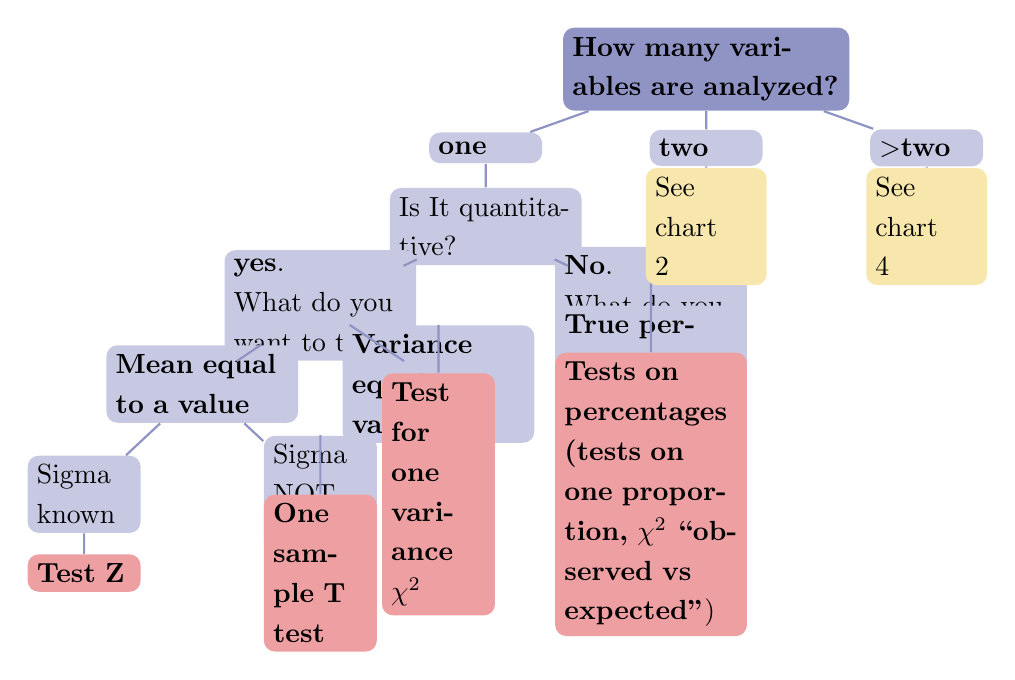
\begin{tikzpicture}[level distance=10mm]
		
                \tikzstyle{every node}=[fill=blocco!50,rounded corners,text width=1.2cm]
                \tikzstyle{edge from parent}=[blocco,thick,draw]
		\tikzstyle{level 1}=[sibling distance=28mm]
  		\tikzstyle{level 2}=[sibling distance=24mm]
  		\tikzstyle{level 3}=[sibling distance=42mm]
  		\tikzstyle{level 4}=[sibling distance=30mm]
		\tikzstyle{level 5}=[level distance=14mm]
		\tikzstyle{level 6}=[level distance=10mm]
                  \node[text width=3.4cm] [fill=blocco]{\textbf{How many variables are analyzed?}}
			child {node {\textbf{one}}
				child {node [text width=2.2cm] {Is It quantitative?}
					child {node [text width=2.2cm]{\textbf{yes}. \\ What do you want to test?}
						child {node[text width=2.2cm] {\textbf{Mean equal to a value}}
							child {node {Sigma known}
								child {node[fill=bloccoFinale!50] {\textbf{Test Z}}}}
							child {node {Sigma NOT known}
								child {node [fill=bloccoFinale!50]{\textbf{One sample T test}}}}}
						child {node [text width=2.2cm]{\textbf{Variance equal to a value}}
							child {node [fill=bloccoFinale!50]{\textbf{Test for one variance} $\chi^2$}}}}
					child {node [text width=2.2cm]{\textbf{No}.\\ What do you want to test?}
						child {node [text width=2.2cm] {\textbf{True percentage equal to a value}}
							child {node[text width=2.2cm] [fill=bloccoFinale!50]{\textbf{Tests on percentages (tests on one proportion, $\chi^2$ ``observed vs expected''}) }}}}}}
			child {node{\textbf{two}}child {node[ text width=1.3cm] [fill=bloccoSospeso!50]{See chart 2}}}
			child {node{ $>$\textbf{two}}child {node[ text width=1.3cm] [fill=bloccoSospeso!50]{See chart 4}}};

         \end{tikzpicture}
\end{tiny}
}

\end{frame}

\livelloA{Chart 2}
\begin{frame}

\onslide<1>{
\begin{tiny}
	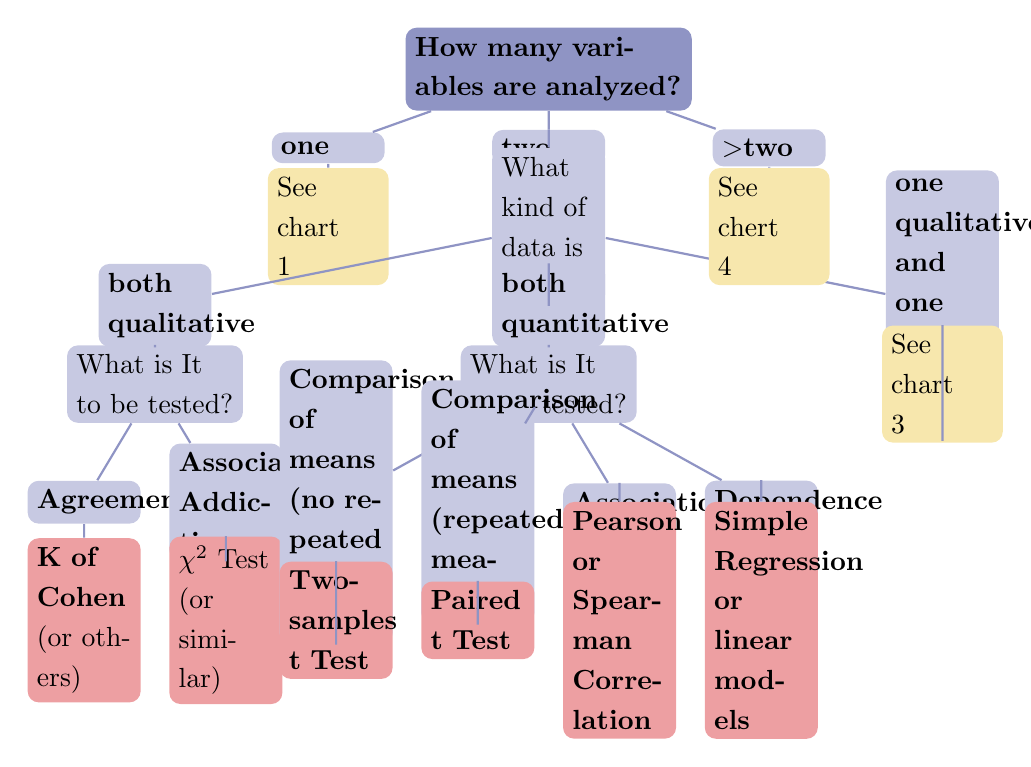
\begin{tikzpicture}[level distance=10mm]
                \tikzstyle{every node}=[fill=blocco!50,rounded corners,text width=1.2cm]
                \tikzstyle{edge from parent}=[blocco,thick,draw]
		\tikzstyle{level 1}=[sibling distance=28mm]
  		\tikzstyle{level 3}=[sibling distance=50mm]
  		\tikzstyle{level 4}=[sibling distance=18mm]
  		\tikzstyle{level 5}=[level distance=15mm]
                  \node [ text width=3.4cm] [fill=blocco]{\textbf{How many variables are analyzed?}}
			child {node{\textbf{one}}child {node [ text width=1.3cm][fill=bloccoSospeso!50]{See chart 1}}}
			child {node {\textbf{two}}
				child {node  {What kind of data is used?}
					child {node {\textbf{both \\ qualitative}}
						child {node [ text width=2cm]{What is It to be tested?}
							child {node {\textbf{Agreement}}
								child {node[fill=bloccoFinale!50] {\textbf{K of Cohen} (or others)}}}
							child {node {\textbf{Association Addiction}}
								child {node [fill=bloccoFinale!50]{\textbf{$\chi^2$} Test\\(or similar)}}}}}
					child {node {\textbf{both \\ quantitative}}
						child {node [ text width=2cm]{What is It to be tested?}
							child {node {\textbf{Comparison of means (no repeated measures)}}
								child {node [fill=bloccoFinale!50]{\textbf{Two-samples t Test}}}}
							child {node {\textbf{Comparison of means \\(repeated measures)}}
								child {node [fill=bloccoFinale!50]{\textbf{Paired t Test}}}}
							child {node {\textbf{Association}}
								child {node [fill=bloccoFinale!50]{\textbf{Pearson or Spearman Correlation}}}}
							child {node {\textbf{Dependence}}
								child {node [fill=bloccoFinale!50]{\textbf{Simple \\ Regression or linear models}}}}}}
					child {node {\textbf{one \\ qualitative \\ and one quantitative}}child {node [ text width=1.3cm] [fill=bloccoSospeso!50]{See chart 3}}}}}
			child {node{$>$\textbf{two}}child {node[ text width=1.3cm] [fill=bloccoSospeso!50]{See chert 4}}};
         \end{tikzpicture}
\end{tiny}
}

\end{frame}


\livelloA{Chart 3}
\begin{frame}

\onslide<1>{
\begin{tiny}
	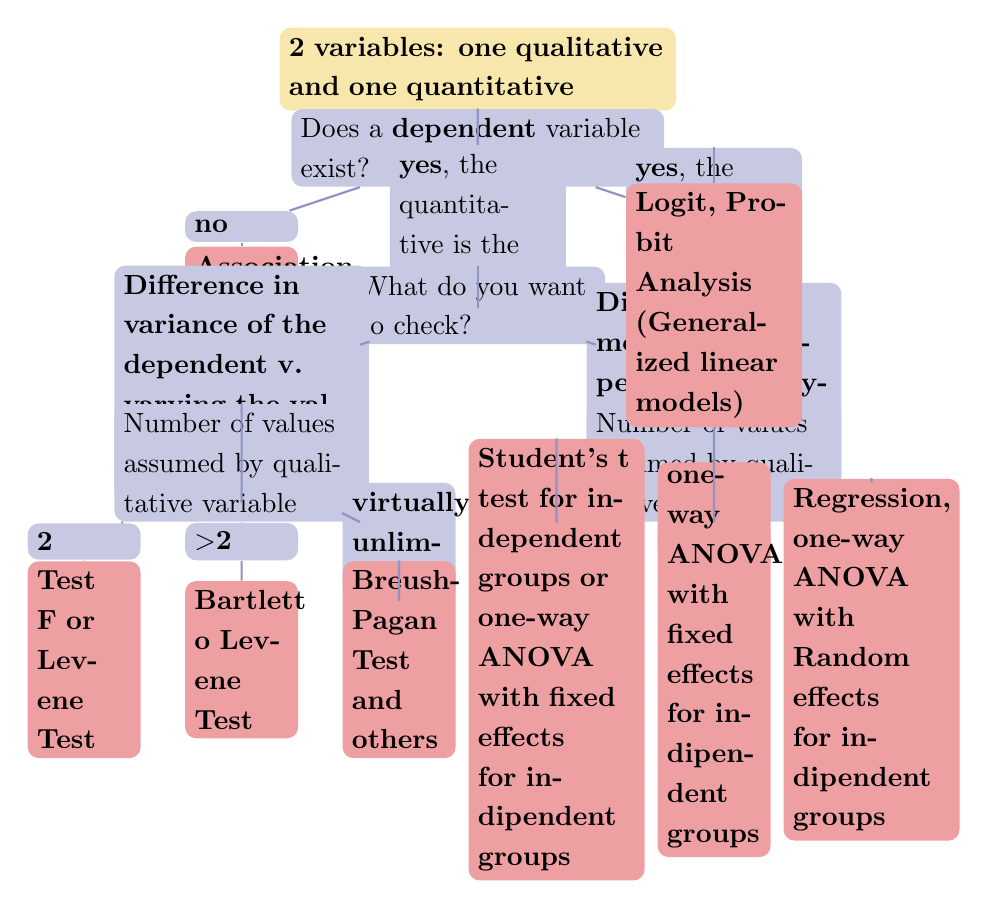
\begin{tikzpicture}[level distance=10mm]
                \tikzstyle{every node}=[fill=blocco!50,rounded corners,text width=1.2cm]
                \tikzstyle{edge from parent}=[blocco,thick,draw]
		\tikzstyle{level 1}=[sibling distance=40mm]
  		\tikzstyle{level 2}=[sibling distance=30mm]
  		\tikzstyle{level 3}=[sibling distance=60mm]
  		\tikzstyle{level 5}=[sibling distance=20mm]
  		\tikzstyle{level 6}=[sibling distance=70mm]
		\tikzstyle{level 6}=[level distance=10mm]
  		\tikzstyle{level 7}=[level distance=15mm]
                  \node[ text width=4.8cm][fill=bloccoSospeso!50] {\textbf{2 variables: one qualitative and one quantitative}}
			child {node [ text width=4.5cm] {Does a \textbf{dependent} variable exist?}
			child {node {\textbf{no}}
				child {node [fill=bloccoFinale!50]{\textbf{Association indexes}}}}
			child {node [ text width=2cm] {\textbf{yes}, the quantitative is the dependent}
				child {node [ text width=3cm]{What do you want to check?}
					child {node[ text width=3cm] {\textbf{Difference in variance of the dependent v. varying the values of the qualitative v.}}
						child {node [ text width=3cm] {Number of values assumed by qualitative variable}
						child {node {\textbf{2}}
							child {node[fill=bloccoFinale!50] {\textbf{Test F or Levene Test}}}}
						child {node {$>$\textbf{2}}
							child {node[fill=bloccoFinale!50] {\textbf{Bartlett o Levene Test}}}}
						child {node {\textbf{virtually unlimited}}
							child {node [fill=bloccoFinale!50]{\textbf{Breush-Pagan Test and others}}}}}}
					child {node [ text width=3cm] {\textbf{Difference in mean of the dependent v. varying the values of the qualitative v.}}
						child {node [ text width=3cm] {Number of values assumed by qualitative variable}
						child {node {\textbf{2}}
							child {node [ text width=2cm][fill=bloccoFinale!50]{\textbf{Student's t test for independent groups or one-way ANOVA with fixed effects for indipendent groups}}}}
						child {node {$>$\textbf{2}}
							child {node[fill=bloccoFinale!50] {\textbf{one-way ANOVA with fixed effects for indipendent groups}}}}
						child {node {\textbf{virtually unlimited}}
							child {node[fill=bloccoFinale!50][ text width=2cm] {\textbf{Regression, one-way ANOVA with Random effects for indipendent groups} }}}}
				}}}
			child {node [ text width=2cm]{\textbf{yes}, the qualitative is the dipendent}
				child {node[fill=bloccoFinale!50] [ text width=2cm] {\textbf{Logit, Probit \\ Analysis (Generalized linear models)}}}}};
         \end{tikzpicture}
\end{tiny}
}
\end{frame}

\livelloA{Chart 4}
\begin{frame}
\onslide<1>{
\begin{tiny}
	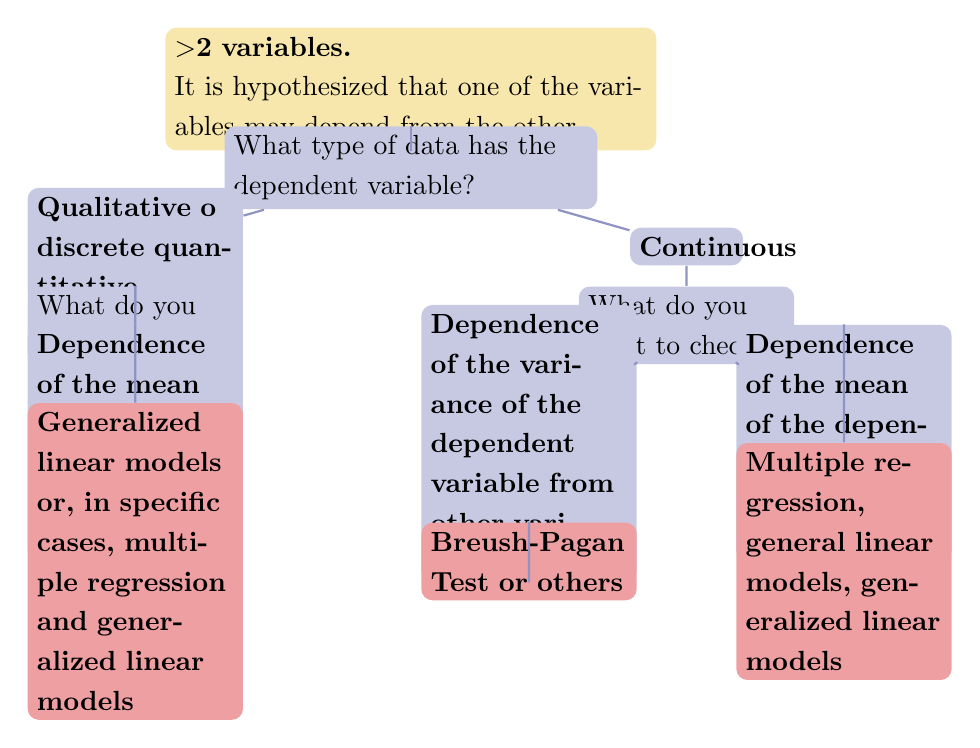
\begin{tikzpicture}[level distance=10mm]
                \tikzstyle{every node}=[fill=blocco!50,rounded corners,text width=1.2cm]
                \tikzstyle{edge from parent}=[blocco,thick,draw]
		\tikzstyle{level 2}=[sibling distance=70mm]
  		\tikzstyle{level 3}=[sibling distance=40mm]
  		\tikzstyle{level 4}=[level distance=15mm]
  		%\tikzstyle{level 3}=[sibling distance=60mm]
                  \node[ text width=6cm][fill=bloccoSospeso!50] {\textbf{$>$2 variables.} \\ It is hypothesized that one of the variables may depend from the other}
			child {node [ text width=4.5cm]{What type of data has the dependent variable?}
				child {node [ text width=2.5cm]{\textbf{Qualitative o discrete quantitative}}
					child {node [ text width=2.5cm] {What do you want to check?}
						child {node [ text width=2.5cm]{\textbf{Dependence of the mean of the dependent variable from other variables}}
							child {node [ text width=2.5cm] [fill=bloccoFinale!50]{\textbf{Generalized linear models or, in specific cases, multiple regression and generalized linear models}}}}}}
				child {node {\textbf{Continuous}}
					child {node [ text width=2.5cm]{What do you want to check?}
						child {node [ text width=2.5cm]{\textbf{Dependence of the variance of the dependent variable from other variables}}
							child {node [ text width=2.5cm][fill=bloccoFinale!50]{\textbf{Breush-Pagan Test or others}}}}
						child {node [ text width=2.5cm]{\textbf{Dependence of the mean of the dependent variable from other variables}}
							child {node [ text width=2.5cm][fill=bloccoFinale!50] {\textbf{Multiple regression,\\  general linear models, generalized linear models}}}}}}};
		\end{tikzpicture}
\end{tiny}
}
\end{frame}





\end{document}
